\documentclass[dutch]{beamer}
\mode<presentation>

%\documentclass[handout]{beamer}
%\usepackage{pgfpages}
%\pgfpagesuselayout{4 on 1}[a4paper,border shrink=5mm,landscape]
%\setbeamertemplate{footline}[frame number]

\usepackage[dutch]{babel}
\usepackage{graphicx}
\usepackage{amssymb, subfigure}
\usepackage{amsthm}
\usepackage[utf8]{inputenc}
\usepackage[normalem]{ulem}
\usepackage{color}
\usepackage{cancel}
%\usepackage{translator}
\usepackage{pgf,tikz}
\usetikzlibrary{arrows}


\swapnumbers\newtheorem{stelling}{Stelling}[section]
\newtheorem{hulpstelling}[stelling]{Hulpstelling}
\newtheorem{gevolg}[stelling]{Gevolg}
\newtheorem{gevolgen}[stelling]{Gevolgen}
\newtheorem{voorbeeld}[stelling]{Voorbeeld}
\newtheorem{voorbeelden}[stelling]{Voorbeelden}
\newtheorem{belangrijkvoorbeeld}[stelling]{Belangrijk voorbeeld}
\newtheorem{belangrijkgevolg}[stelling]{Belangrijk gevolg}
\newtheorem{belangrijkegevolgen}[stelling]{Belangrijke gevolgen}
\newtheorem{opmerking}[stelling]{Opmerking}
\newtheorem{opmerkingen}[stelling]{Opmerkingen}
\newtheorem{definitie}[stelling]{Definitie}
\newtheorem{toepassing}[stelling]{Toepassing}
\newtheorem{oefeningen}[stelling]{Oefeningen}
\newtheorem{definities}[stelling]{Definities}
\newtheorem{oefening}[stelling]{Oefening}
\newtheorem{notatie}[stelling]{Notatie}
\newtheorem{onderzoeksvraag}{Onderzoeksvraag}

\graphicspath{{afbeeldingen/}}

%\usetheme{Copenhagen}
%\usecolortheme{dolphins}
%rgb ---> 0.3,0.5,0.7 mooi blauw
\usetheme{antibes}
%\definecolor{mycolor}{RGB}{48,96,102}
%\definecolor{mycolor2}{RGB}{63,125,133}
%\setbeamercolor*{palette primary}{use=structure,fg=white,bg=mycolor}
\setbeamertemplate{navigation symbols}{}

\definecolor{darkblue}{rgb}{0,0,0.6}


\title[Vullen van Vlakken en Volumes]{Vullen van Vlakken en Volumes}
\author[Lien Lambert \& Pieter Pareit \& Jordy Vanpoucke ]{Lien Lambert \\Pieter Pareit \\Jordy Vanpoucke}
\date{\tiny 15 mei 2012}

\begin{document}

\frame{
%\begin{figure}[t]
%	\flushleft
%		\includegraphics[scale=0.1]{logo.jpg}
%\end{figure}
\titlepage}

%\frame{
%\tableofcontents 
%}

\begin{frame}

\begin{enumerate}
	\item Inleiding
	  \begin{itemize}
	    \item Motivatie
	    \item Doelgroep en voorkennis
    \end{itemize}
  \item Overzicht van de lessen
    \begin{itemize}
	    \item Les 1: Inleiding
	    \item Les 2 + 3: Vullen van vierkanten, perfecte vierkanten, puzzelen met vierkanten en hun toepassingen
	    \item Les 4+5+6: Tweedimensionale stapelproblemen en het dienbladenprobleem
	    \item Les 7+8: Driedimensionale stapelproblemen, het bolstapelprobleem van Kepler
    \end{itemize}
\end{enumerate}
\end{frame}

\section{Inleiding}
%\subsection{Motivatie}
\begin{frame}
\frametitle{Motivatie: het waarom?}
\pause
\begin{figure}[h]
\centering
\only<2>{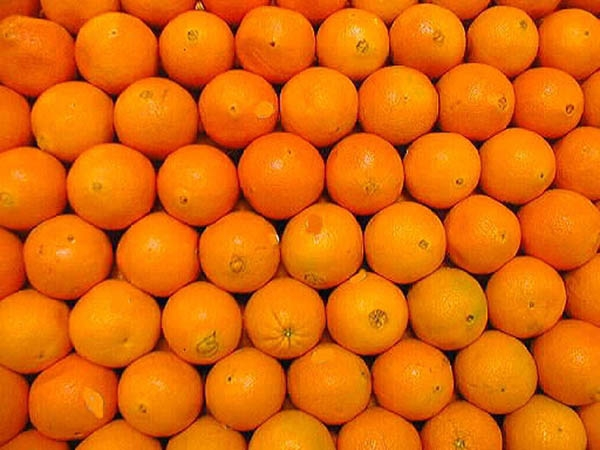
\includegraphics[height=4.8cm]{oranges}}
\pause
\only<3>{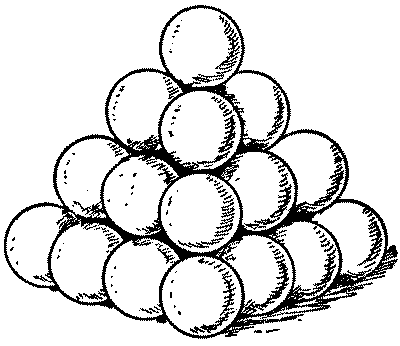
\includegraphics[height=4.8cm]{cannonballs}}
\pause
\only<4>{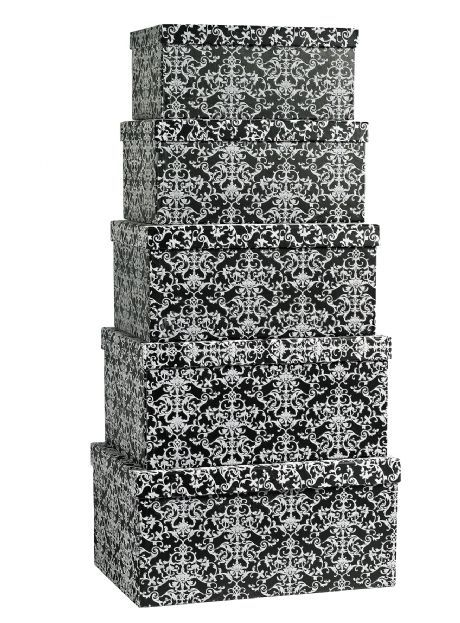
\includegraphics[height=4.8cm]{dozen}}
\pause
\only<5>{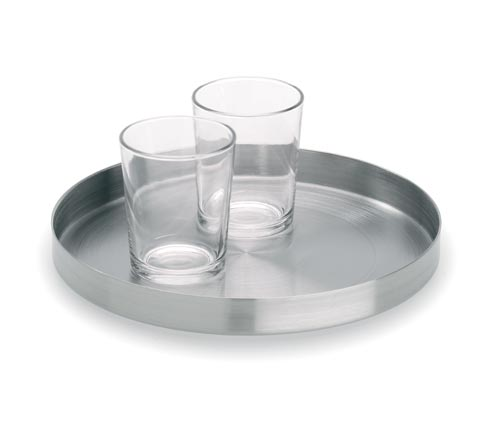
\includegraphics[height=4.8cm]{dienblad}}
\pause
\only<6>{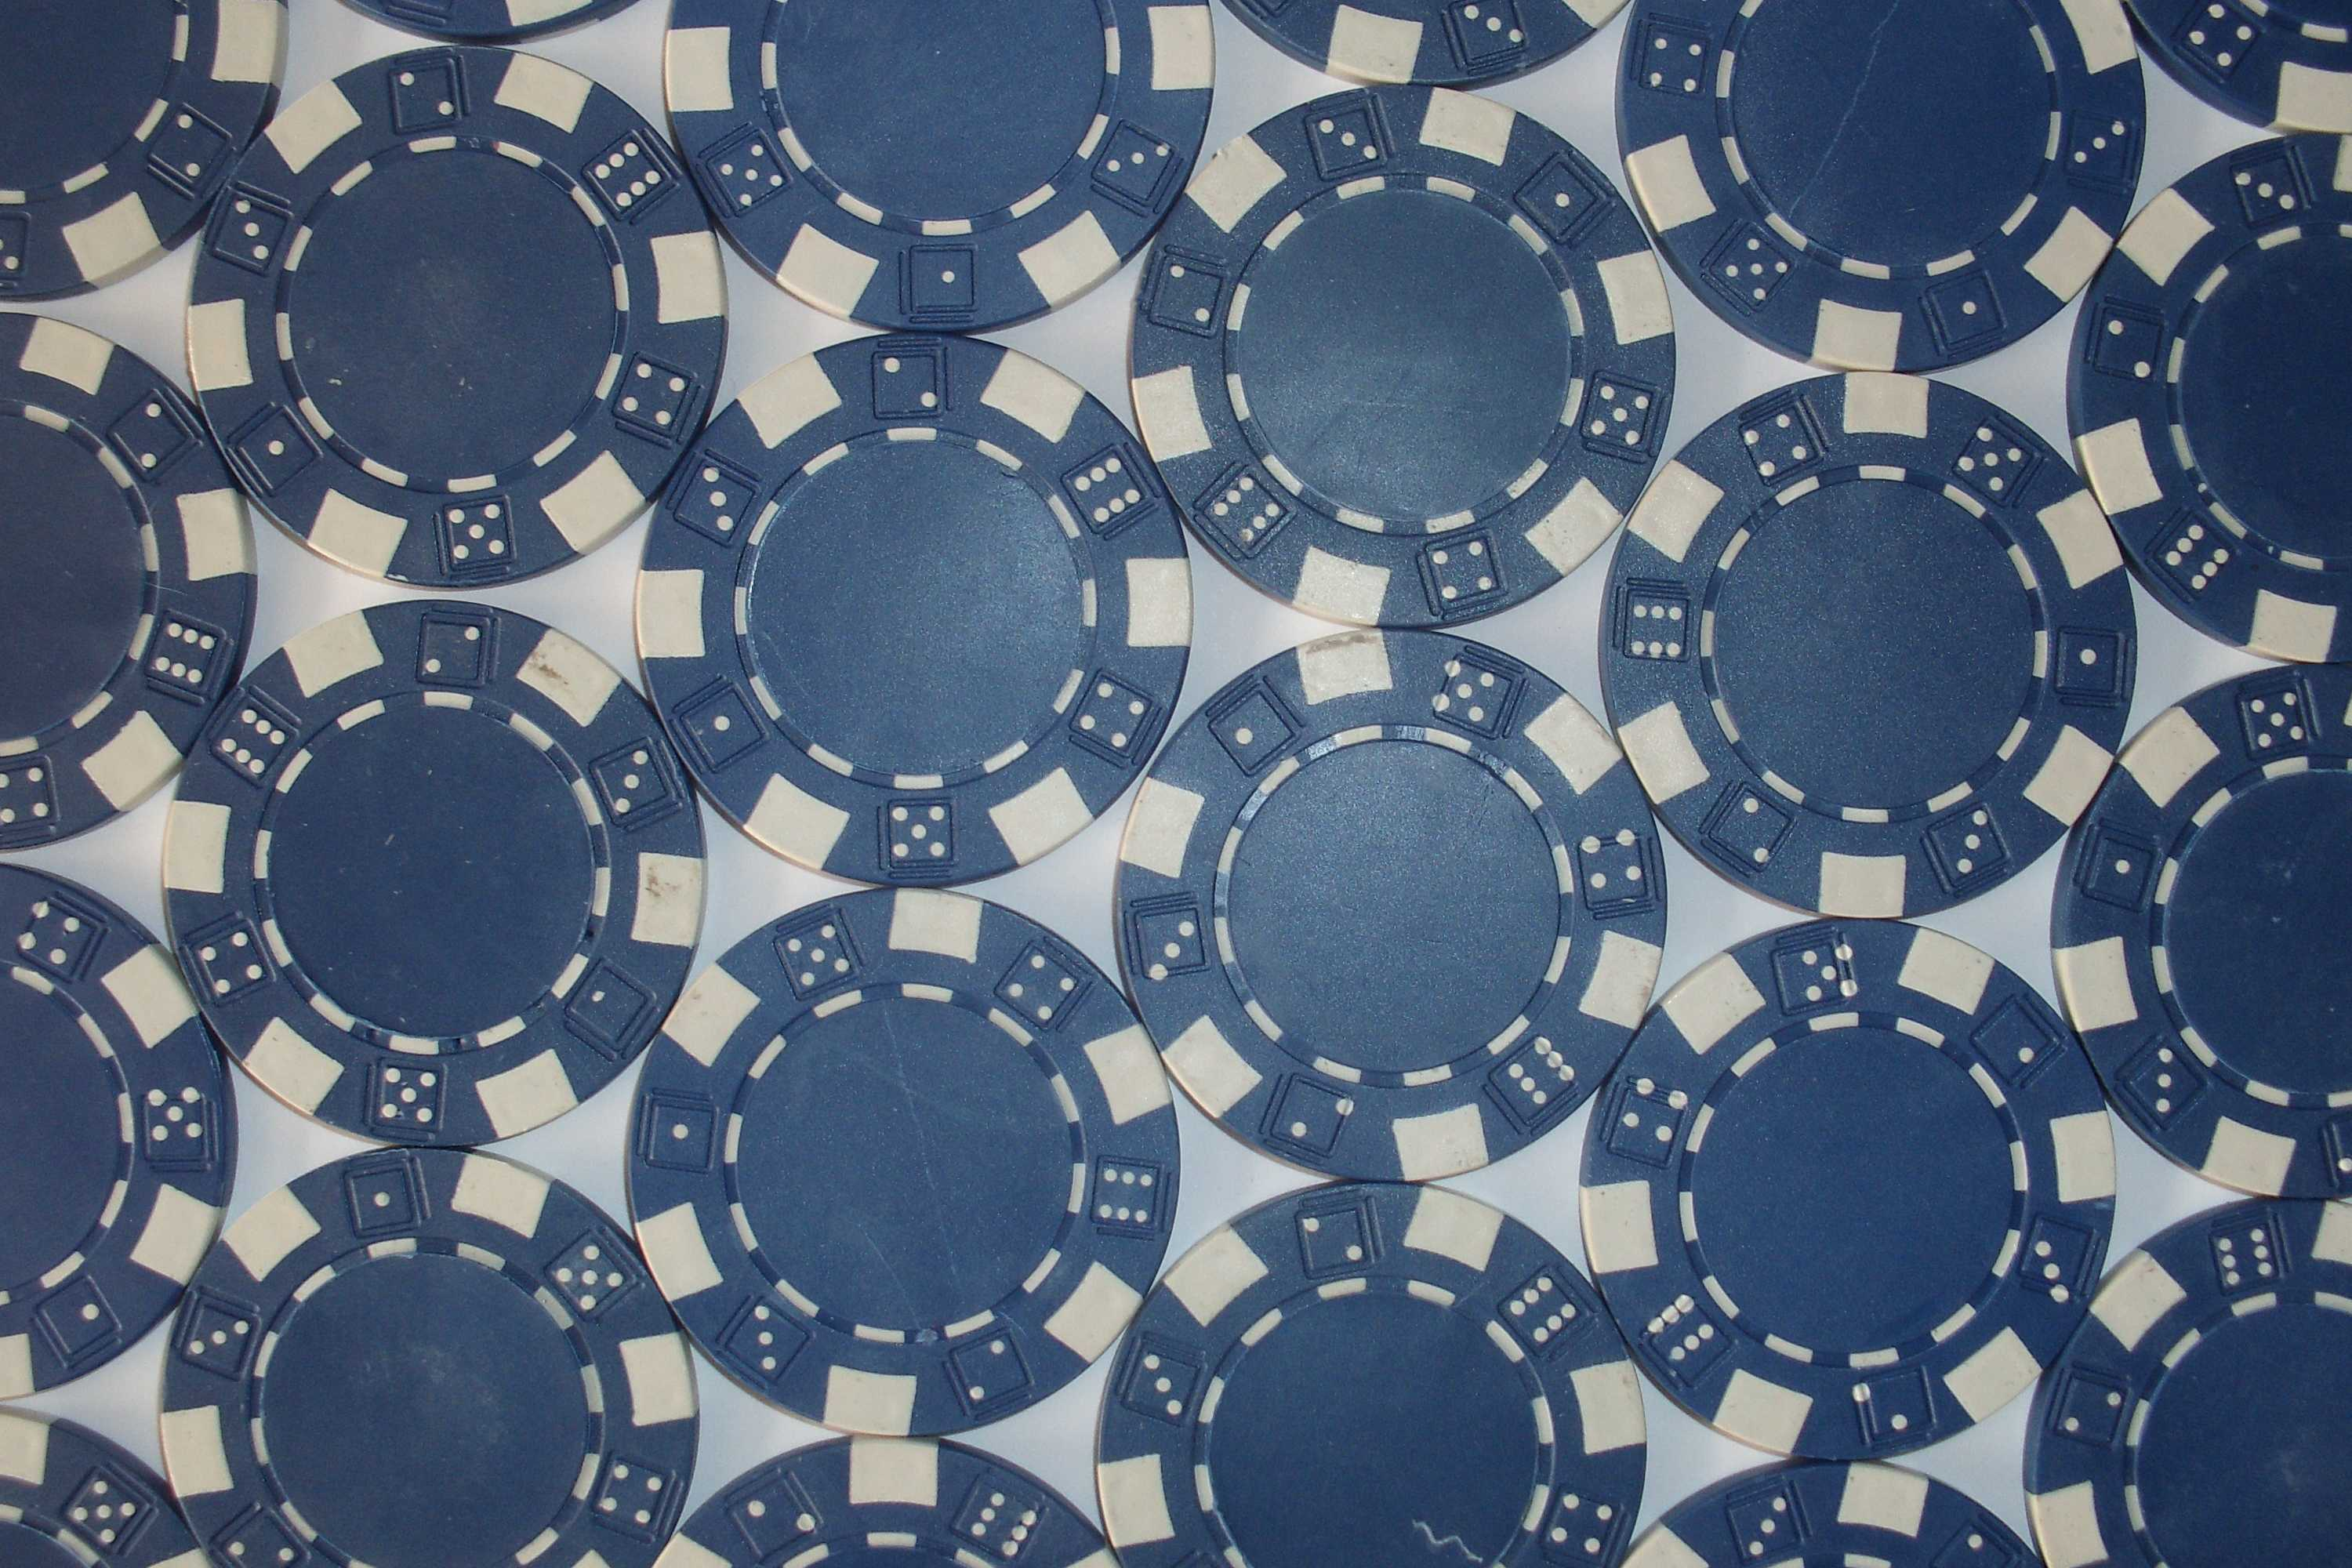
\includegraphics[height=4.8cm]{jetons_hex}}
\end{figure}
\end{frame}


%\subsection{Doelgroep en voorkennis}

\begin{frame}
\frametitle{Doelgroep}
\pause
\begin{itemize}
\item $2^{de}$ graad ASO
\pause
\item Ook $3^{de}$ graad ASO\pause, maar \ldots
\end{itemize}
\end{frame}


\begin{frame}
\frametitle{Voorkennis}
\pause
\begin{itemize}
\item verschillende vakgebieden
\pause
\begin{itemize}
\item getallenleer en algebra
\item re\"{e}le functies
\item meetkunde
\end{itemize}
\pause
\item `voorkennis'
\end{itemize}
\end{frame}

\section{Lessenreeks}

\begin{frame}
\begin{center}
\textbf{\Large{Vullen van Vlakken en Volumes}}
\end{center}
\end{frame}

\begin{frame}
{Overzicht van de lessen}
\begin{list}{\quad}{}
\item {\color{blue}Les 1: Inleiding}
\item Les 2: Vullen van vierkanten met kleinere vierkanten en zo tot Perfecte Vierkanten komen
\item Les 3: Puzzelen met vierkanten en rechthoeken om vergelijkingen op te lossen
\item Les 4: Kennismaking met tweedimensionale stapelproblemen en hiermee experimenteren
\item Les 5: Het dienbladenprobleem: experimenteren en effectief berekenen
\item Les 6: Het dienbladenprobleem: berekenen, bewijzen en besluiten
\item Les 7: Kanonskogels stapelen
\item Les 8: Vervolg kanonskogels en het bolstapelprobleem van Kepler
\end{list}
\end{frame}


\subsection{Les 1: Inleiding}
\begin{frame}
\begin{itemize}
\item De leerlingen kennen de definities van een vlakvulling, een complete vlakvulling en een optimale vlakvullling.
\item De leerlingen kunnen in groep komen tot bevindingen over het compleet vullen van een oneindig groot vlak.
\item De leerlingen kunnen bewijzen dat een betegeling van een oneindig groot vlak met regelmatige veelhoeken enkel lukt met regelmatige driehoeken, regelmatige vierhoeken en regelmatige zeshoeken.
\item De leerlingen kennen stapelproblemen.
\item De leerlingen kunnen zelfstandig op zoek gaan naar meer informatie over het lesonderwerp.
\item De leerlingen kunnen in groep samenwerken om enkele raadsels op te lossen.
\end{itemize}
\end{frame}

\begin{frame}
{Overzicht van de lessen}
\begin{list}{\quad}{}
\item Les 1: Inleiding
\item {\color{blue}Les 2: Vullen van vierkanten met kleinere vierkanten en zo tot Perfecte Vierkanten komen}
\item Les 3: Puzzelen met vierkanten en rechthoeken om vergelijkingen op te lossen
\item Les 4: Kennismaking met tweedimensionale stapelproblemen en hiermee experimenteren
\item Les 5: Het dienbladenprobleem: experimenteren en effectief berekenen
\item Les 6: Het dienbladenprobleem: berekenen, bewijzen en besluiten
\item Les 7: Kanonskogels stapelen
\item Les 8: Vervolg kanonskogels en het bolstapelprobleem van Kepler
\end{list}
\end{frame}

\subsection{Les 2: Vullen van vierkanten met kleinere vierkanten en zo tot Perfecte Vierkanten komen}

\begin{frame}
\begin{itemize}
\item De leerlingen kunnen een een vierkant met kleinere vierkanten vullen van de zelfde grootte, om zo een algemene formule die de maximale effici\"{e}ntie bepaald, te vinden.
\item De leerlingen weten wat een perfect vierkant van orde $n$ is.
\item De leerlingen kunnen een ondergrens zoeken voor de orde van het perfect vierkant door redeneren.
\item De leerlingen zien in dat een perfect vierkant dat gedraaid of gespiegeld wordt geen ander perfect vierkant oplevert. Hiervoor leren de leerlingen het begrip isomorfisme.
\item De leerlingen beseffen dat het vinden van \'{e}\'{e}n perfect vierkant leidt tot het vinden van een oneindig aantal perfecte vierkanten. 
\item De leerlingen kunnen een bewijs uit het ongerijmde opstellen om een eigenschap te bewijzen over perfecte vierkanten.
\item De leerlingen kunnen hun resultaten en definities in verband met perfecte vierkanten uitbreiden naar \'{e}\'{e}n en drie dimensies.
\end{itemize}
\end{frame}

\begin{frame}
  \frametitle{Les 2: Vullen van vierkanten met kleinere vierkanten}
  \framesubtitle{Resultaten: vullen van een vierkant met kleinere vierkanten}
  \begin{columns}
    \begin{column}{0.5\textwidth}
      \definecolor{cqcqcq}{rgb}{0.75,0.75,0.75}
\begin{tikzpicture}[scale=0.4,line cap=round,line join=round,>=triangle 45,x=1.0cm,y=1.0cm]
\draw [color=cqcqcq,dash pattern=on 2pt off 2pt, xstep=1.0cm,ystep=1.0cm] (-0.5,-0.5) grid (10.5,10.5);
\clip(-0.5,-0.5) rectangle (10.5,10.5);
\filldraw[line width=1.6pt,fill=black,fill opacity=0.1] (0,0) -- (10,0) -- (10,10) -- (0,10) -- cycle;
\filldraw[fill=black,fill opacity=0.1] (0,0) -- (3,0) -- (3,3) -- (0,3) -- cycle;
\filldraw[fill=black,fill opacity=0.1] (3,0) -- (6,0) -- (6,3) -- (3,3) -- cycle;
\filldraw[fill=black,fill opacity=0.1] (6,0) -- (9,0) -- (9,3) -- (6,3) -- cycle;
\filldraw[fill=black,fill opacity=0.1] (0,3) -- (3,3) -- (3,6) -- (0,6) -- cycle;
\filldraw[fill=black,fill opacity=0.1] (3,3) -- (6,3) -- (6,6) -- (3,6) -- cycle;
\filldraw[fill=black,fill opacity=0.1] (6,3) -- (9,3) -- (9,6) -- (6,6) -- cycle;
\filldraw[fill=black,fill opacity=0.1] (0,6) -- (3,6) -- (3,9) -- (0,9) -- cycle;
\filldraw[fill=black,fill opacity=0.1] (3,6) -- (6,6) -- (6,9) -- (3,9) -- cycle;
\filldraw[fill=black,fill opacity=0.1] (6,6) -- (9,6) -- (9,9) -- (6,9) -- cycle;
\end{tikzpicture}

    \end{column}
    \begin{column}{0.5\textwidth}
    \begin{itemize}
      \item Voorbeeld:
      \begin{align*}
        10^2  &= (3\cdot 3 + 1)^2\\
        \Leftrightarrow 100   &= (3\cdot 3)^2 + 2\cdot 3\cdot 3\cdot 1 + 1^2\\
        \Leftrightarrow 100   &= 81 + 19
      \end{align*}
      \pause
      \item Algemeen:
      \begin{align*}
         a^2  &= (q\cdot d + r)^2\\
        \Leftrightarrow a^2   &= (q\cdot d)^2 + 2\cdot q\cdot d\cdot r + r^2
      \end{align*}
      {\tiny met $a$ de zijde van het grote vierkante, $d$ de zijde van de kleine vierkanten, $q$ het aantal keer we $d$ in $a$ krijgen en $r$ de rest die dan nog overblijft}
    \end{itemize}
    \end{column}
  \end{columns}  
\end{frame}

\begin{frame}
  \frametitle{Les 2: Vullen van vierkanten met kleinere vierkanten}
  \framesubtitle{Alles over perfecte vierkanten}
  \begin{columns}
    \begin{column}{0.4\textwidth}
      \only<1-2>{{\small
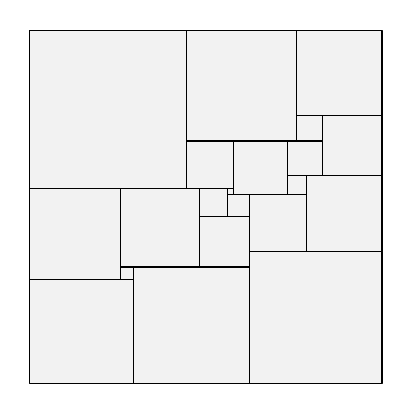
\begin{tikzpicture}[scale=0.04,line cap=round,line join=round,>=triangle 45,x=1.0cm,y=1.0cm]
\clip(-0.5,-0.5) rectangle (113,113);
\filldraw[fill=black,fill opacity=0.05] (0,0) -- (33,0) -- (33,33) -- (0,33) -- cycle;
\filldraw[fill=black,fill opacity=0.05] (33,0) -- (70,0) -- (70,37) -- (33,37) -- cycle;
\filldraw[fill=black,fill opacity=0.05] (70,0) -- (112,0) -- (112,42) -- (70,42) -- cycle;
\filldraw[fill=black,fill opacity=0.05] (0,33) -- (29,33) -- (29,62) -- (0,62) -- cycle;
\filldraw[fill=black,fill opacity=0.05] (29,33) -- (33,33) -- (33,37) -- (29,37) -- cycle;
\filldraw[fill=black,fill opacity=0.05] (0,62) -- (50,62) -- (50,112) -- (0,112) -- cycle;
\filldraw[fill=black,fill opacity=0.05] (29,62) -- (29,37) -- (54,37) -- (54,62) -- cycle;
\filldraw[fill=black,fill opacity=0.05] (54,37) -- (70,37) -- (70,53) -- (54,53) -- cycle;
\filldraw[fill=black,fill opacity=0.05] (70,42) -- (88,42) -- (88,60) -- (70,60) -- cycle;
\filldraw[fill=black,fill opacity=0.05] (88,42) -- (112,42) -- (112,66) -- (88,66) -- cycle;
\filldraw[fill=black,fill opacity=0.05] (54,53) -- (63,53) -- (63,62) -- (54,62) -- cycle;
\filldraw[fill=black,fill opacity=0.05] (63,53) -- (70,53) -- (70,60) -- (63,60) -- cycle;
\filldraw[fill=black,fill opacity=0.05] (63,60) -- (65,60) -- (65,62) -- (63,62) -- cycle;
\filldraw[fill=black,fill opacity=0.05] (82,60) -- (88,60) -- (88,66) -- (82,66) -- cycle;
\filldraw[fill=black,fill opacity=0.05] (65,60) -- (82,60) -- (82,77) -- (65,77) -- cycle;
\filldraw[fill=black,fill opacity=0.05] (50,62) -- (65,62) -- (65,77) -- (50,77) -- cycle;
\filldraw[fill=black,fill opacity=0.05] (50,112) -- (50,77) -- (85,77) -- (85,112) -- cycle;
\filldraw[fill=black,fill opacity=0.05] (82,77) -- (82,66) -- (93,66) -- (93,77) -- cycle;
\filldraw[fill=black,fill opacity=0.05] (93,66) -- (112,66) -- (112,85) -- (93,85) -- cycle;
\filldraw[fill=black,fill opacity=0.05] (85,77) -- (93,77) -- (93,85) -- (85,85) -- cycle;
\filldraw[fill=black,fill opacity=0.05] (85,85) -- (112,85) -- (112,112) -- (85,112) -- cycle;
\end{tikzpicture}
}
}
      \only<3->{{\small
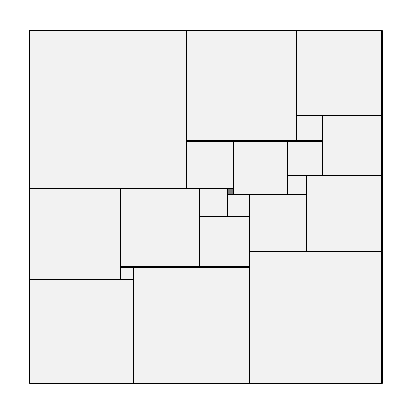
\begin{tikzpicture}[scale=0.04,line cap=round,line join=round,>=triangle 45,x=1.0cm,y=1.0cm]
\clip(-0.5,-0.5) rectangle (113,113);
\filldraw[fill=black,fill opacity=0.05] (0,0) -- (33,0) -- (33,33) -- (0,33) -- cycle;
\filldraw[fill=black,fill opacity=0.05] (33,0) -- (70,0) -- (70,37) -- (33,37) -- cycle;
\filldraw[fill=black,fill opacity=0.05] (70,0) -- (112,0) -- (112,42) -- (70,42) -- cycle;
\filldraw[fill=black,fill opacity=0.05] (0,33) -- (29,33) -- (29,62) -- (0,62) -- cycle;
\filldraw[fill=black,fill opacity=0.05] (29,33) -- (33,33) -- (33,37) -- (29,37) -- cycle;
\filldraw[fill=black,fill opacity=0.05] (0,62) -- (50,62) -- (50,112) -- (0,112) -- cycle;
\filldraw[fill=black,fill opacity=0.05] (29,62) -- (29,37) -- (54,37) -- (54,62) -- cycle;
\filldraw[fill=black,fill opacity=0.05] (54,37) -- (70,37) -- (70,53) -- (54,53) -- cycle;
\filldraw[fill=black,fill opacity=0.05] (70,42) -- (88,42) -- (88,60) -- (70,60) -- cycle;
\filldraw[fill=black,fill opacity=0.05] (88,42) -- (112,42) -- (112,66) -- (88,66) -- cycle;
\filldraw[fill=black,fill opacity=0.05] (54,53) -- (63,53) -- (63,62) -- (54,62) -- cycle;
\filldraw[fill=black,fill opacity=0.05] (63,53) -- (70,53) -- (70,60) -- (63,60) -- cycle;
\filldraw[fill=black,fill opacity=0.5] (63,60) -- (65,60) -- (65,62) -- (63,62) -- cycle;
\filldraw[fill=black,fill opacity=0.05] (82,60) -- (88,60) -- (88,66) -- (82,66) -- cycle;
\filldraw[fill=black,fill opacity=0.05] (65,60) -- (82,60) -- (82,77) -- (65,77) -- cycle;
\filldraw[fill=black,fill opacity=0.05] (50,62) -- (65,62) -- (65,77) -- (50,77) -- cycle;
\filldraw[fill=black,fill opacity=0.05] (50,112) -- (50,77) -- (85,77) -- (85,112) -- cycle;
\filldraw[fill=black,fill opacity=0.05] (82,77) -- (82,66) -- (93,66) -- (93,77) -- cycle;
\filldraw[fill=black,fill opacity=0.05] (93,66) -- (112,66) -- (112,85) -- (93,85) -- cycle;
\filldraw[fill=black,fill opacity=0.05] (85,77) -- (93,77) -- (93,85) -- (85,85) -- cycle;
\filldraw[fill=black,fill opacity=0.05] (85,85) -- (112,85) -- (112,112) -- (85,112) -- cycle;
\end{tikzpicture}
}
}
    \end{column}
    \begin{column}{0.6\textwidth}
    {\scriptsize
      \begin{itemize}
        \item Een {\bf perfect vierkant} is een vierkant dat opgedeeld kan worden in een eindig aantal kleinere vierkanten waarvan geen twee dezelfde grootte hebben.
        \item De {\bf orde} van een perfect vierkant is het aantal kleinere vierkanten dat het bevat.
        \pause
        \item Het vierkant heeft $8$ symmetrie�n, de dihedrale groep $D4$, dus ��n oplossing leidt tot 8 isomorfe oplossingen.
          \begin{center}
            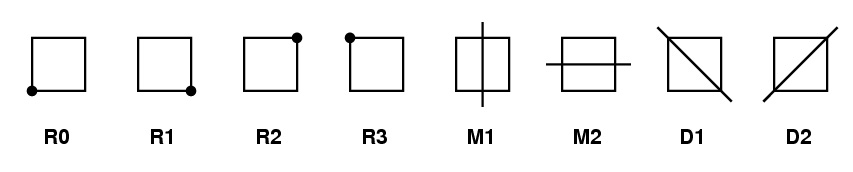
\includegraphics[width=0.8\textwidth]{dih4}
          \end{center}
        \pause
        \item Door het perfecte vierkant te hertekenen binnen het kleinste vierkantje construeren we nieuwe perfecte vierkanten.
        \pause
        \item Een {\bf fractaal} is een meetkundige figuur die zelfgelijkend is. 
      \end{itemize}
    }
    \end{column}
  \end{columns}  
\end{frame}

\begin{frame}
  \frametitle{Les 2: Vullen van vierkanten met kleinere vierkanten}
  \framesubtitle{Eigenschap kleinste vierkantje in een perfect vierkant}
  \begin{columns}
    \begin{column}{0.5\textwidth}
      %\only<1>{\definecolor{cccccc}{rgb}{0.6,0.6,0.6}
\begin{tikzpicture}[scale=0.3, line cap=round,line join=round,>=triangle 45,x=1.0cm,y=1.0cm]
\clip(45,32) rectangle (75,61);
\draw [line width=1.2pt, color=cccccc] (65,32) -- (65,61);
\filldraw[line width=1.2pt,fill=black,fill opacity=0.1] (54,59.12) -- (63,59.12) -- (63,50.12) -- (54,50.12) -- cycle;
\filldraw[line width=1.2pt,fill=black,fill opacity=0.1] (63,59.12) -- (70,59.12) -- (70,52.12) -- (63,52.12) -- cycle;
\filldraw[line width=1.2pt,fill=black,fill opacity=0.15] (63,52.12) -- (65,52.12) -- (65,50.12) -- (63,50.12) -- cycle;
\filldraw[line width=1.2pt,fill=black,fill opacity=0.1] (50,50.12) -- (65,50.12) -- (65,35.12) -- (50,35.12) -- cycle;
\end{tikzpicture}
}
      \definecolor{cccccc}{rgb}{0.6,0.6,0.6}
\begin{tikzpicture}[scale=0.3, line cap=round,line join=round,>=triangle 45,x=1.0cm,y=1.0cm]
\clip(45,32) rectangle (75,61);
\draw [line width=1.2pt, color=cccccc] (65,32) -- (65,61);
\filldraw[line width=1.2pt,fill=black,fill opacity=0.1] (54,59.12) -- (63,59.12) -- (63,50.12) -- (54,50.12) -- cycle;
\filldraw[line width=1.2pt,fill=black,fill opacity=0.1] (63,59.12) -- (70,59.12) -- (70,52.12) -- (63,52.12) -- cycle;
\filldraw[line width=1.2pt,fill=black,fill opacity=0.15] (63,52.12) -- (65,52.12) -- (65,50.12) -- (63,50.12) -- cycle;
\filldraw[line width=1.2pt,fill=black,fill opacity=0.1] (50,50.12) -- (65,50.12) -- (65,35.12) -- (50,35.12) -- cycle;
\end{tikzpicture}

    \end{column}
    \begin{column}{0.5\textwidth}
    {\scriptsize
      \begin{stelling}
      Het kleinste vierkantje in een perfect vierkant kan nooit aan de rand liggen.
      \end{stelling}
      {\tiny
        \begin{list}{}{\leftmargin=0pt}
          \pause
          \item Uit het ongerijmde.
          \item Veronderstel dat het kleinste vierkantje in een perfect vierkant op de rand ligt.
          \pause
          \item Hoeveel vierkantjes liggen dan nog rond het kleinste vierkantje?
          \item Wat weten we over de vierkantjes die rond het kleinste vierkantje liggen?
          \pause
          \item Dus \'e\'en van de vierkantjes komt over de rand!
          \pause
          \item Dus we hebben geen perfect vierkant, een strijdigheid!
          \item Dus het kleinste vierkantje kan niet op de rand liggen!
        \end{list}
      }
    }
    \end{column}
  \end{columns}  
\end{frame}


\begin{frame}
{Overzicht van de lessen}
\begin{list}{\quad}{}
\item Les 1: Inleiding
\item Les 2: Vullen van vierkanten met kleinere vierkanten en zo tot Perfecte Vierkanten komen
\item {\color{blue}Les 3: Puzzelen met vierkanten en rechthoeken om vergelijkingen op te lossen}
\item Les 4: Kennismaking met tweedimensionale stapelproblemen en hiermee experimenteren
\item Les 5: Het dienbladenprobleem: experimenteren en effectief berekenen
\item Les 6: Het dienbladenprobleem: berekenen, bewijzen en besluiten
\item Les 7: Kanonskogels stapelen
\item Les 8: Vervolg kanonskogels en het bolstapelprobleem van Kepler
\end{list}
\end{frame}

\subsection{Les 3: Puzzelen met vierkanten en rechthoeken om vergelijkingen op te lossen}

\begin{frame}
\begin{itemize}
  \item De leerlingen kunnen voor hen gekende methoden, uit de algebra, gebruiken om problemen op te lossen, i.h.b. de methode voor het oplossen van een vierkantsvergelijking.
  \item De leerlingen kunnen dan dezelfde problemen op een meetkundige manier oplossen.
  \item De leerlingen beseffen dat er een link is tussen algebra en meetkunde.
  \item De leerlingen hebben een idee hoe het oplossen van derdegraadsvergelijkingen historisch is gegroeid.
\end{itemize}
\end{frame}

\begin{frame}
{Overzicht van de lessen}
\begin{list}{\quad}{}
\item Les 1: Inleiding
\item Les 2: Vullen van vierkanten met kleinere vierkanten en zo tot Perfecte Vierkanten komen
\item Les 3: Puzzelen met vierkanten en rechthoeken om vergelijkingen op te lossen
\item {\color{blue}Les 4: Kennismaking met tweedimensionale stapelproblemen en hiermee experimenteren}
\item Les 5: Het dienbladenprobleem: experimenteren en effectief berekenen
\item Les 6: Het dienbladenprobleem: berekenen, bewijzen en besluiten
\item Les 7: Kanonskogels stapelen
\item Les 8: Vervolg kanonskogels en het bolstapelprobleem van Kepler
\end{list}
\end{frame}

\subsection{Les 4: Kennismaking met tweedimensionale stapelproblemen en hiermee experimenteren}

\begin{frame}
\begin{itemize}
\item De leerlingen beseffen dat je een tafel niet volledig kan bedekken met cirkels en dat we daarom op zoek kunnen gaan naar de optimale configuratie, namelijk het hexagonaal rooster.
\item De leerlingen weten wat een voronoicel is en kunnen hiermee de effici\"{e}ntie van een rooster berekenen.
\item De leerlingen kunnen de oppervlakte van een driehoek, rechthoek, zeshoek en cirkel berekenen.
\item De leerlingen kunnen a.d.h.v. een geogebra-applet of door te experimenteren met jetons of munten de effici\"{e}ntie van dienbladen bepalen.
\item De leerlingen kunnen de effici\"{e}ntie voor eenvoudige voorbeelden uitrekenen.
\item De leerlingen ontwikkelen meetkundig inzicht.
\end{itemize}
\end{frame}

\begin{frame}
{Overzicht van de lessen}
\begin{list}{\quad}{}
\item Les 1: Inleiding
\item Les 2: Vullen van vierkanten met kleinere vierkanten en zo tot Perfecte Vierkanten komen
\item Les 3: Puzzelen met vierkanten en rechthoeken om vergelijkingen op te lossen
\item Les 4: Kennismaking met tweedimensionale stapelproblemen en hiermee experimenteren
\item {\color{blue}Les 5: Het dienbladenprobleem: experimenteren en effectief berekenen}
\item Les 6: Het dienbladenprobleem: berekenen, bewijzen en besluiten
\item Les 7: Kanonskogels stapelen
\item Les 8: Vervolg kanonskogels en het bolstapelprobleem van Kepler
\end{list}
\end{frame}

\subsection{Les 5: Het dienbladenprobleem: experimenteren en effectief berekenen}

\begin{frame}
\begin{itemize}
\item De leerlingen kunnen a.d.h.v. een Geogebra-applet of door te experimenteren met jetons(of munten) de effici\"{e}ntie van dienbladen bepalen.
\item De leerlingen kunnen functioneel gebruik maken van ICT.
\item De leerlingen kunnen de effici\"{e}ntie voor eenvoudige voorbeelden uitrekenen.
\item De leerlingen kunnen vanuit een figuur meetkundig inzicht verwerven en hierdoor problemen vereenvoudigen.
\item De leerlingen kunnen de meetkundige interpretatie van de goniometrische formules functioneel gebruiken, i.h.b. voor projecties.
\end{itemize}
\end{frame}

\begin{frame}
{Overzicht van de lessen}
\begin{list}{\quad}{}
\item Les 1: Inleiding
\item Les 2: Vullen van vierkanten met kleinere vierkanten en zo tot Perfecte Vierkanten komen
\item Les 3: Puzzelen met vierkanten en rechthoeken om vergelijkingen op te lossen
\item Les 4: Kennismaking met tweedimensionale stapelproblemen en hiermee experimenteren
\item Les 5: Het dienbladenprobleem: experimenteren en effectief berekenen
\item {\color{blue}Les 6: Het dienbladenprobleem: berekenen, bewijzen en besluiten}
\item Les 7: Kanonskogels stapelen
\item Les 8: Vervolg kanonskogels en het bolstapelprobleem van Kepler
\end{list}
\end{frame}

\subsection{Les 6: Het dienbladenprobleem: berekenen, bewijzen en besluiten}

\begin{frame}
\begin{itemize}
\item De leerlingen beseffen dat men uit experimenteren belangrijke informatie kan halen en beseffen ook het belang van bewijzen.
\item De leerlingen kunnen aan de hand van een stappenplan het bewijs zelf verwerven.
\item De leerlingen kunnen de effici\"{e}ntie van ingewikkelde configuraties berekenen.
\item De leerlingen kunnen vorige berekeningen gebruiken om ingewikkelde configuraties te vereenvoudigen.
\item De leerlingen kunnen uit experimentele resultaten conclusies trekken over de meest effici\"{e}nte dienbladen, en kunnen ook (mogelijke) verklaringen geven.
\end{itemize}
\end{frame}

\begin{frame}
{Overzicht van de lessen}
\begin{list}{\quad}{}
\item Les 1: Inleiding
\item Les 2: Vullen van vierkanten met kleinere vierkanten en zo tot Perfecte Vierkanten komen
\item Les 3: Puzzelen met vierkanten en rechthoeken om vergelijkingen op te lossen
\item Les 4: Kennismaking met tweedimensionale stapelproblemen en hiermee experimenteren
\item Les 5: Het dienbladenprobleem: experimenteren en effectief berekenen
\item Les 6: Het dienbladenprobleem: berekenen, bewijzen en besluiten
\item {\color{blue}Les 7: Kanonskogels stapelen}
\item Les 8: Vervolg kanonskogels en het bolstapelprobleem van Kepler
\end{list}
\end{frame}

\subsection{Les 7: Kanonskogels stapelen}

\begin{frame}
\begin{itemize}
\item De leerlingen weten wat het bolstapelprobleem inhoudt.
\item De leerlingen kunnen het aantal kanonskogels in een (regelmatige) piramide met vierkant en driehoekig grondvlak met $n$ lagen experimenteel berekenen.
\item De leerlingen kunnen vanuit een gegeven rij het recursief en/of expliciet voorschrift geven.
\item De leerlingen kunnen door het doordacht experimenteren bepaalde vragen over combinaties van piramides onderzoeken.
\item De leeringen kunnen een bewijs geven voor de som van de eerste $n$ kwadraten.
\item De leerlingen kunnen op een analoge wijze het bewijs geven voor de som van de eerst $n$ driehoeksgetallen.
\end{itemize}
\end{frame}

\begin{frame}
{Overzicht van de lessen}
\begin{list}{\quad}{}
\item Les 1: Inleiding
\item Les 2: Vullen van vierkanten met kleinere vierkanten en zo tot Perfecte Vierkanten komen
\item Les 3: Puzzelen met vierkanten en rechthoeken om vergelijkingen op te lossen
\item Les 4: Kennismaking met tweedimensionale stapelproblemen en hiermee experimenteren
\item Les 5: Het dienbladenprobleem: experimenteren en effectief berekenen
\item Les 6: Het dienbladenprobleem: berekenen, bewijzen en besluiten
\item Les 7: Kanonskogels stapelen
\item {\color{blue}Les 8: Vervolg kanonskogels en het bolstapelprobleem van Kepler}
\end{list}
\end{frame}

\subsection{Les 8: Vervolg kanonskogels en het bolstapelprobleem van Kepler}

\begin{frame}
\begin{itemize}
\item De leerlingen kunnen door het doordacht experimenteren bepaalde vragen over combinaties van piramides onderzoeken.
\item De leerlingen kunnen vanuit een voorbeeld komen tot een algemene formule en dit ook bewijzen, al dan niet met behulp van de leerkracht.
\item De leerlingen weten wat het bolstapelprobleem inhoudt.
\item De leerlingen beseffen dat het vinden van een bewijs soms vele jaren kan duren.
\item De leerlingen beseffen dat de controle van een bewijs soms geen evidentie is, bijvoorbeeld omdat een deel van het bewijs door een computerprogramma geleverd wordt.
\item De leerlingen weten wat een `kissing number' is.
\end{itemize}
\end{frame}


\end{document}

